% Author: Alfredo Sánchez Alberca (asalber@ceu.es}
% !TEX program = xelatex
\documentclass[aspectratio=149,10pt,t]{beamer}
%-------------------------------------------------------------------------------
% GENERAL PACKAGES
%-------------------------------------------------------------------------------
% Language
\usepackage{polyglossia}
\setdefaultlanguage{spanish}
% Maths
\usepackage{amsmath} % Math symbols and environments
\usepackage{amsfonts}
\usepackage{amssymb}
% Tables
\usepackage{array}
\usepackage{multirow}
% Graphics
\usepackage{graphicx}
\usepackage{tikz}
\usetikzlibrary{positioning}


% Colors
\definecolor{blueceu}{RGB}{0,164,227}
\definecolor{greenceu}{RGB}{194,205,24}
\definecolor{redceu}{RGB}{238,50,36}
\definecolor{purpleceu}{RGB}{169,78,145}
\definecolor{greyceu}{RGB}{117,117,97}
\definecolor{darkgrey}{RGB}{40,40,50}
\definecolor{softblueceu}{RGB}{193,225,246}
\setbeamercolor{structure}{fg=blueceu}
\setbeamercolor{normal text}{fg=darkgrey}
\hypersetup{colorlinks, urlcolor=purpleceu}

%-------------------------------------------------------------------------------
% FONTS
%-------------------------------------------------------------------------------
\usepackage{fontspec}
\setmainfont[Ligatures=TeX]{TeX Gyre Pagella}
\usepackage{unicode-math}
\setmathfont[math-style=ISO,bold-style=ISO,vargreek-shape=TeX]{TeX Gyre Pagella Math}
% Creative common icons
\usepackage[scale=1.5]{ccicons}

%-------------------------------------------------------------------------------
% CONFIGURATION
%-------------------------------------------------------------------------------
\setbeamersize{text margin left=.5cm, text margin right=.5cm} % Defines margin sizes
\beamertemplatenavigationsymbolsempty % Hide navitation bar
\usefonttheme[onlymath]{serif} % Math text in serif
\setbeamertemplate{blocks}[rounded] % Blocks with rounded corners
%\setbeamercolor{block title}{bg=RoyalBlue!10} % Color of block title
%\setbeamercolor{block body}{bg=RoyalBlue!10} % Color of block body


%-------------------------------------------------------------------------------
% DOCUMENT
%-------------------------------------------------------------------------------
\begin{document}
%---------------------------------------------------------------------SLIDE----
\begin{frame}[c]
\vspace{1.5cm}

\begin{center}
\structure{\LARGE {\textbf{Ejercicios de Estadística}}}
\bigskip

\large
\begin{tabular}{rl}
Temas: & \structure{Probabilidad}\\
Titulaciones: & \structure{Todas}
\end{tabular}

\bigskip
Alfredo Sánchez Alberca\\
\url{asalber@ceu.es}\\
\url{http://aprendeconalf.es}\\


\includegraphics[scale=0.2]{../img/logo_uspceu}

\bigskip
{\color{darkgrey}\ccbyncsaeu}
\end{center}
\end{frame}


%----------------------------------------------------------------------SLIDE----
\begin{frame}[c]
	\large
	En una asignatura se hacen dos exámenes parciales a lo largo del curso.
	El primer parcial lo aprobaron el 60\% de los alumnos y el segundo parcial lo aprobaron el 68\%.
	Del grupo de alumnos que aprobaron el primer parcial, el 80\% de ellos aprobaron el segundo.
	Si se elige un alumno al azar, calcular:
	\begin{enumerate}
	  \item Probabilidad de que no haya aprobado ningún parcial.
	  \item Probabilidad de que haya aprobado el primer parcial si no ha aprobado el segundo.
  \end{enumerate}
\end{frame}


%----------------------------------------------------------------------SLIDE----
\begin{frame}
	\begin{columns}
		\begin{column}[T]{0.6\textwidth}
			En una asignatura se hacen dos exámenes parciales a lo largo del curso.
			El primer parcial lo aprobaron el 60\% de los alumnos y el segundo parcial lo aprobaron el 68\%.
			Del grupo de alumnos que aprobaron el primer parcial, el 80\% de ellos aprobaron el segundo.
		\end{column}
		\begin{column}[T]{0.4\textwidth}
			\structure{Datos}\\
			$A_1 \equiv$ Aprobar el primer parcial\\
			$A_2 \equiv$ Aprobar el segundo parcial\\
			$P(A_1)=0.6$\\
			$P(A_2)=0.68$\\
			$P(A_2|A_1)=0.8$
		\end{column}
	\end{columns}
\end{frame}

%----------------------------------------------------------------------SLIDE----
\begin{frame}
	\begin{columns}
		\begin{column}[T]{0.5\textwidth}
			\begin{enumerate}
			  \item Probabilidad de que no haya aprobado ningún parcial.
		  \end{enumerate}
		\end{column}
		\begin{column}[T]{0.5\textwidth}
			\structure{Datos}
			\medskip

			\resizebox{\textwidth}{!}{
			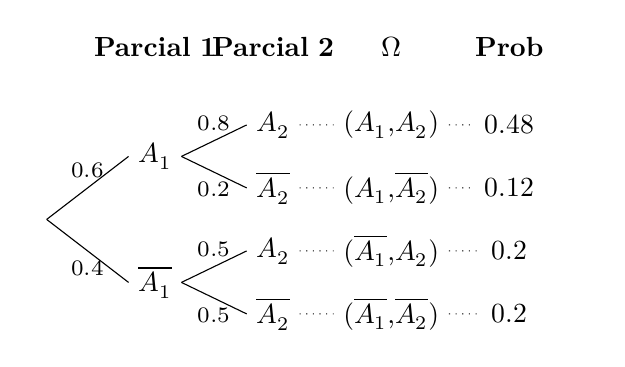
\begin{tikzpicture}[
			grow'=right,
			level 1/.style ={level distance=1.5cm, sibling distance=1.6cm, parent anchor=east, child anchor=west},
			level 2/.style ={level distance=1.5cm, sibling distance=0.8cm},
			level 3/.style ={level distance=1.5cm, sibling distance=0.8cm, dotted},
			level 4/.style ={level distance=1.5cm, sibling distance=0.8cm, dotted},
			prob/.style={font=\footnotesize,above}
			]

			\node (root) {}
				child {node {$A_1$}
					child {node {$A_2$}
						child {node{($A_1$,$A_2$)}
							child {node{$0.48$}}
						}
						edge from parent node[prob] {$0.8$}
					}
					child {node {$\overline{A_2}$}
						child {node{($A_1$,$\overline{A_2}$)}
							child {node{$0.12$}}
						}
						edge from parent node[prob,below] {$0.2$}
					}
					edge from parent node[prob] {$0.6$}
				}
				child {node {$\overline{A_1}$}
			   		child {node {$A_2$}
						child {node{($\overline{A_1}$,$A_2$)}
							child {node{$0.2$}}
						}
						edge from parent node[prob] {$0.5$}
					}
					child {node {$\overline{A_2}$}
						child {node{($\overline{A_1}$,$\overline{A_2}$)}
							child {node{$0.2$}}
						}
						edge from parent node[prob,below] {$0.5$}
					}
					edge from parent node[prob,below] {$0.4$}
				};

			\begin{scope}[every node/.style={text width=2cm, align=center, anchor=center, font=\bfseries,}]
			\node[above= 0.5cm of root-1-1-1-1] (labels-level) {Prob};
			\node[at =(labels-level-|root-1-1-1)] {$\Omega$};
			\node[at =(labels-level-|root-1-1)] {Parcial 2};
			\node[at =(labels-level-|root-1)] {Parcial 1};
			\end{scope}
		\end{tikzpicture}}
		\end{column}
	\end{columns}
\end{frame}


%----------------------------------------------------------------------SLIDE----
\begin{frame}
	\begin{columns}
		\begin{column}[T]{0.6\textwidth}
			\begin{enumerate}
			  \item Probabilidad de que no haya aprobado ningún parcial.
		  \end{enumerate}
		\end{column}
		\begin{column}[T]{0.4\textwidth}
			\structure{Datos}\\
			$A_1 \equiv$ Aprobar el primer parcial\\
			$A_2 \equiv$ Aprobar el segundo parcial\\
			$P(A_1)=0.6$\\
			$P(A_2)=0.68$\\
			$P(A_2|A_1)=0.8$
		\end{column}
	\end{columns}
\end{frame}


%----------------------------------------------------------------------SLIDE----
\begin{frame}
	\begin{columns}
		\begin{column}[T]{0.5\textwidth}
			\begin{enumerate}
			  \item[2.] Probabilidad de que haya aprobado el primer parcial si no ha aprobado el segundo.
		  \end{enumerate}
		\end{column}
		\begin{column}[T]{0.5\textwidth}
			\structure{Datos}
			\medskip

			\resizebox{\textwidth}{!}{
			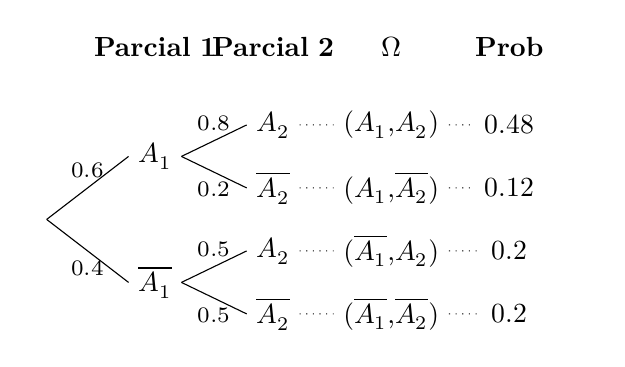
\begin{tikzpicture}[
			grow'=right,
			level 1/.style ={level distance=1.5cm, sibling distance=1.6cm, parent anchor=east, child anchor=west},
			level 2/.style ={level distance=1.5cm, sibling distance=0.8cm},
			level 3/.style ={level distance=1.5cm, sibling distance=0.8cm, dotted},
			level 4/.style ={level distance=1.5cm, sibling distance=0.8cm, dotted},
			prob/.style={font=\footnotesize,above}
			]

			\node (root) {}
				child {node {$A_1$}
					child {node {$A_2$}
						child {node{($A_1$,$A_2$)}
							child {node{$0.48$}}
						}
						edge from parent node[prob] {$0.8$}
					}
					child {node {$\overline{A_2}$}
						child {node{($A_1$,$\overline{A_2}$)}
							child {node{$0.12$}}
						}
						edge from parent node[prob,below] {$0.2$}
					}
					edge from parent node[prob] {$0.6$}
				}
				child {node {$\overline{A_1}$}
			   		child {node {$A_2$}
						child {node{($\overline{A_1}$,$A_2$)}
							child {node{$0.2$}}
						}
						edge from parent node[prob] {$0.5$}
					}
					child {node {$\overline{A_2}$}
						child {node{($\overline{A_1}$,$\overline{A_2}$)}
							child {node{$0.2$}}
						}
						edge from parent node[prob,below] {$0.5$}
					}
					edge from parent node[prob,below] {$0.4$}
				};

			\begin{scope}[every node/.style={text width=2cm, align=center, anchor=center, font=\bfseries,}]
			\node[above= 0.5cm of root-1-1-1-1] (labels-level) {Prob};
			\node[at =(labels-level-|root-1-1-1)] {$\Omega$};
			\node[at =(labels-level-|root-1-1)] {Parcial 2};
			\node[at =(labels-level-|root-1)] {Parcial 1};
			\end{scope}
		\end{tikzpicture}}
		\end{column}
	\end{columns}
\end{frame}


%----------------------------------------------------------------------SLIDE----
\begin{frame}
	\begin{columns}
		\begin{column}[T]{0.6\textwidth}
			\begin{enumerate}
			  \item[2.] Probabilidad de que haya aprobado el primer parcial si no ha aprobado el segundo.
		  \end{enumerate}
		\end{column}
		\begin{column}[T]{0.4\textwidth}
			\structure{Datos}\\
			$A_1 \equiv$ Aprobar el primer parcial\\
			$A_2 \equiv$ Aprobar el segundo parcial\\
			$P(A_1)=0.6$\\
			$P(A_2)=0.68$\\
			$P(A_2|A_1)=0.8$
		\end{column}
	\end{columns}
\end{frame}

\end{document}
